\chapter{Entwurf}\label{chapter:entwurf}

Dieses Kapitel beschäftigt sich mit allen Modulen des Projektes. Unter anderem wird sowohl der Aufbau als auch die Zusammenschaltung mehrerer Module aus der elektrotechnischen Sicht beschrieben, welche in der \autoref{fig:aufbau} grafisch dargestellt wurde.

%%%%%%%%%%%%%%%%%%%%%%%%%%%%%%%%%%%%%%%%%%%%%%%%%%%%%%%%%%%%%%%%%%%%%%%%%%%%%%%
\section{Optokoppler-Modul}

Eine einfache Methode zur Messung der Frequenz eines kontinuierlich-sinusförmigen Signals mit Hilfe eines Mikrocontrollers ist die Digitalisierung dieses Signals, damit die steigenden bzw. fallenden Flanken aufgezählt werden kann. Um dieses sinusförmige Signal zu digitalisieren, wird hier ein \textbf{Optokoppler} benutzt, der ein (Halbleiter-)Bauelement und vor allem in der Nachrichten-Übertragungstechnik sehr nutzbar ist. \smallskip \smallskip

% !!! http://www.renesas.eu/products/opto/technology/ac/index.jsp
Der Optokoppler dient der Signalübertragung zwischen zwei galvanisch vollständig getrennten Stromkreisen in einem gemeinsamen Gehäuse \cite{Mikrocontroller:Optokoppler}. In einem Optokoppler bzw. Gabelkoppler befinden sich ein Lichtsender (\textit{Led}) und ein Lichtempfänger (\textit{Fototransistor}). Die Funktionsweise des Optokopplers ist die Übersetzung von einer sinusförmigen Eingangsspannung zu einer rechteckförmigen Ausgangsspannung \cite{Tietze2002}. Das heißt, dass der Strom am Ausgang über den Fototransistor nur dann fließt, wenn die positive Halbwelle den Lichtsender erreicht. Zusätzlich zu dieser Diode für die positive Halbwelle wird eine Diode für die negative Halbwelle im Eingangsbereich benötigt. In dieser Arbeit findet eine Spannungsquelle im Eingangsbereich mit 10 V (AC) und eine Spannungsquelle im Ausgangsbereich mit 5 V (DC), wie in der \autoref{fig:optokoppler} zu sehen ist.  

\begin{figure}[htbp]
	\centering
	\fbox{
		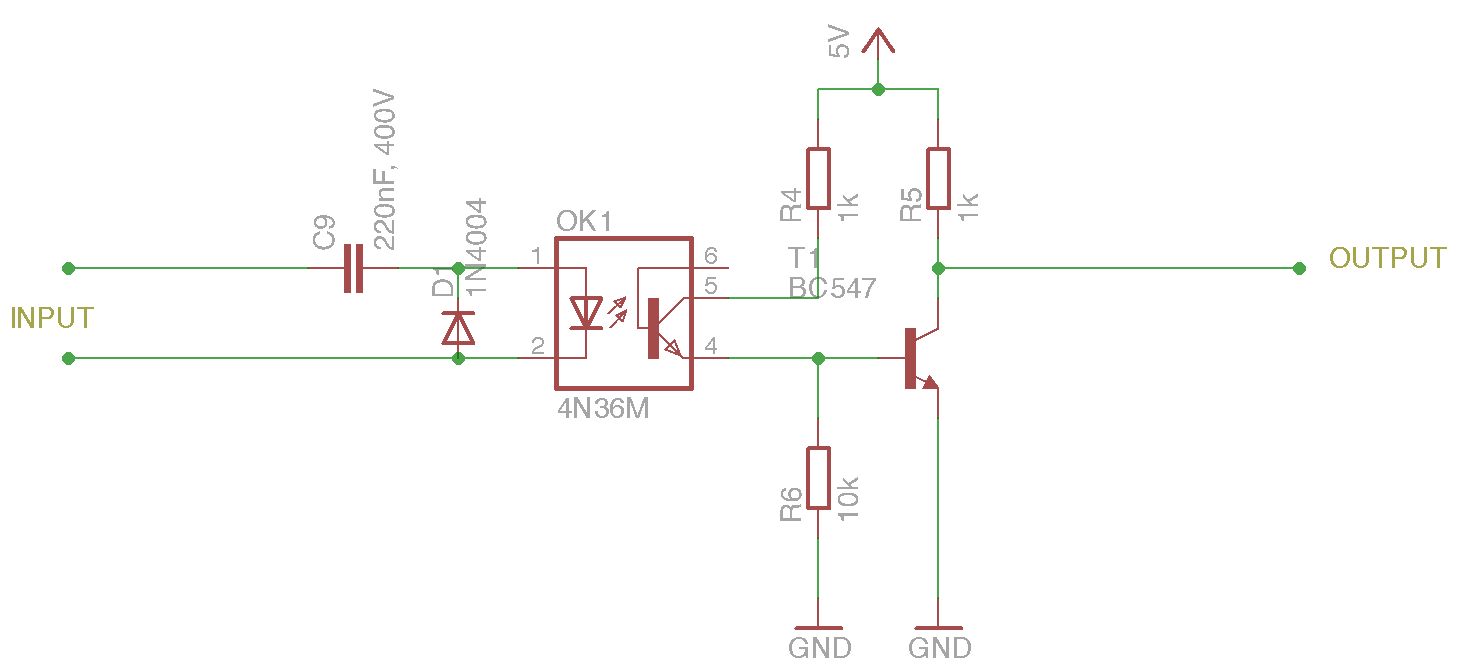
\includegraphics[width=450px,height=203px]{pictures/optokoppler.png}
	}
	\caption{Optokoppler-Modul}\label{fig:optokoppler}
\end{figure}

%%%%%%%%%%%%%%%%%%%%%%%%%%%%%%%%%%%%%%%%%%%%%%%%%%%%%%%%%%%%%%%%%%%%%%%%%%%%%%%
\section{Netzteil-Modul}

Sowohl für das Atmel-Modul als auch für das Netzwerk-Modul wird ein Netzteil benötigt, damit diese an das Netz angeschlossen werden können. Jedes Modul hat eine spezifische Versorgungsspannung. Die Versorgungsspannung beim Atmel-Modul liegt bei $5$ Volt ($\pm 10 \%$) und beim Netzwerk-Modul bei $3.3$ Volt ($\pm 10 \%$). \smallskip \smallskip

Wie in der \autoref{fig:netzteil} zu sehen ist, wird das Atmel-Modul mit $5$ Volt Spannung und das Netzwerk-Modul mit $3.3$ Volt Spannung verbunden.

\begin{figure}[htbp]
	\centering
	\fbox{
		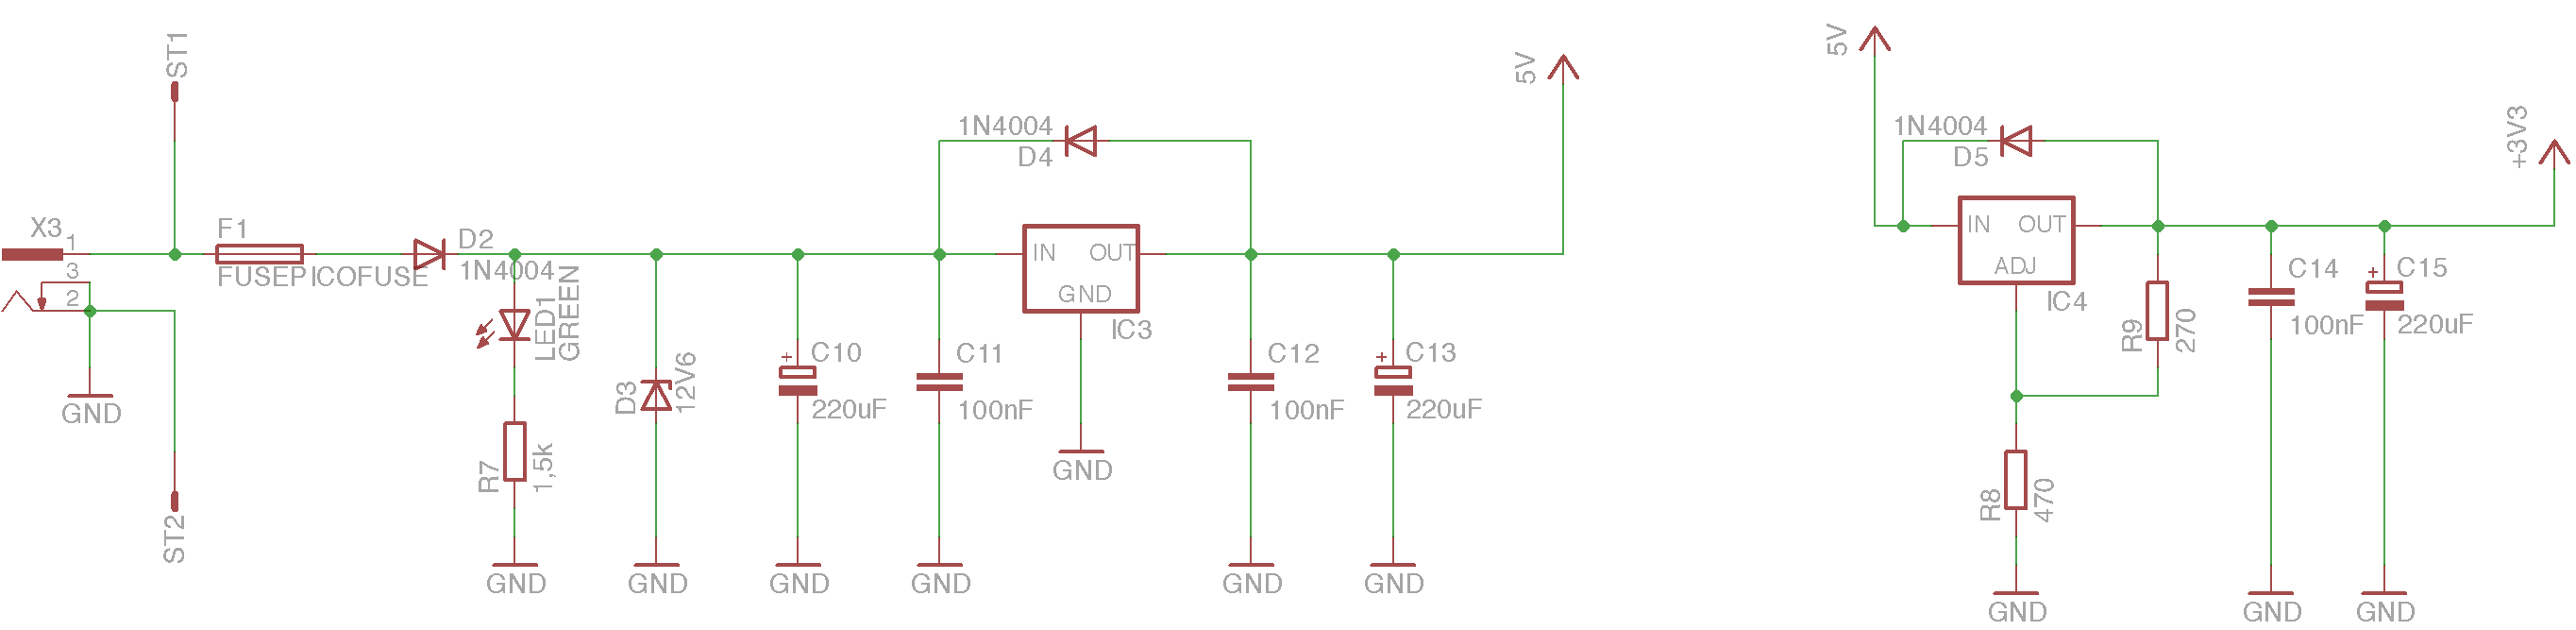
\includegraphics[width=450px,height=110px]{pictures/netzteil.png}
	}
	\caption{Netzteil-Modul}\label{fig:netzteil}
\end{figure}

%%%%%%%%%%%%%%%%%%%%%%%%%%%%%%%%%%%%%%%%%%%%%%%%%%%%%%%%%%%%%%%%%%%%%%%%%%%%%%%
\section{AVR JTAGICE mkII}\label{sec:atmel:jtag}

Um einen funktionierenden Mikrocontroller zu erzielen, muss dieser Mikrocontroller mit einem Entwicklungswerkzeug bzw. mit einem Programmer programmiert werden. Es wurde für diese Arbeit ein Entwicklungswerkzeug vom Firma \textit{ATMEL Corporation} ausgewählt, nämlich \textbf{AVR JTAGICE mkII} \cite{Mikrocontroller:JTAGICEmkII} (siehe \autoref{fig:jtagicemkII}). Dieses Entwicklungswerkzeug bietet die Möglichkeit für das ''On-Chip-Debugging\footnote{On-Chip-Debugging dient die Möglichkeit, mögliche Fehler im Programmcode direkt auf dem Chip zur Laufzeit zu debuggen bzw. zu finden.}'' und die Programmierung über JTAG für alle AVR 8-bit RISC-Mikrocontrollern. Die JTAG-Schnittstelle wurde für ein Test-Access-Port (\textit{TAP}) entwickelt und als \textit{IEEE 1149.1} im Jahr 1990 standardisiert. 

\begin{figure}[htbp]
	\centering
	\fbox{
		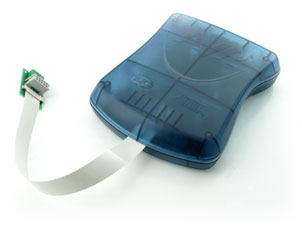
\includegraphics[width=266px,height=200px]{pictures/JTAGICEmkII.jpg}
	}
	\caption[AVR JTAGICE mkII]{AVR JTAGICE mkII \cite{Mikrocontroller:JTAGICE:guide}}\label{fig:jtagicemkII}
\end{figure}

Der JTAGICE-Programmer wird zwischen Entwicklungs- und Zielplattform geschaltet. Er übermittelt somit die Kommunikation zwischen dem Rechner und dem AVR-Mikrocontroller. An den Rechner wird der JTAG-Programmer über ein USB-Kabel angeschlossen und verbraucht keine zusätzliche Versorgungsspannung. An den Mikrocontroller wird der JTAG-Programmer direkt zu den AVR-Pins angeschlossen. Die Pinbelegungen und ihre Beschreibungen sind in der \autoref{fig:jtag}, die Verdrahtung zwischen dem AVR JTAGICE mkII und dem ATMEL-Mikrocontroller in der \autoref{fig:jtag_atmel} beschrieben. 

\begin{table}[htbp]
	\centering
	\begin{tabular}{ |c|c|c|p{9cm}| } \hline
		\textbf{Pin} & \textbf{Signal} & \textbf{I/O} & \textbf{Beschreibung} \\
		\hline
		1 & TCK & Output & Test-Clock, Taktsignal aus JTAGICE mkII zu JTAG-PORT des Ziel-Controllers \\ \hline
		2 & GND & - & Erde \\ \hline
		3 & TDO & Input & Test-Data-Output, Data-Signal aus JTAG-Port des Ziel-Controllers zu JTAGICE mkII \\ \hline
		4 & $V_{ref}$ & Input & Referenzspannung  \\ \hline
		5 & TMS & Output & Auswahl des Testmodes aus JTAGICE mkII zu JTAG-PORT des Ziel-Controllers \\ \hline
		6 & nSRST & OUT-/Input & Zur Steuerung und zur Überwachung über RESET-Pin des Ziel-Controllers\\ \hline
		7 & - & - & nicht verbunden \\ \hline
		8 & nTRST & NC (Output) & nicht verbunden \\ \hline
		9 & TDI & Output &  Test-Data-Input, Data-Signal aus JTAGICE mkII zu JTAG-PORT des Ziel-Controllers \\ \hline
		10 & GND & - & Erde \\ \hline
	\end{tabular}
	\caption{PIN-Belegungen von JTAG-Schnittstelle und ihre Beschreibungen}\label{fig:jtag}
\end{table}

\begin{table}[htbp]
\centering
\begin{tabular}{ |c|c|c|c| }
  \hline
  \multicolumn{2}{|c|}{\textbf{JTAGICE mkII}} & \multicolumn{2}{|c|}{\textbf{ATMega16}}\\ 
  \hline
  TCK & PIN 1& PC2 (PIN 24) & TCK \\
  GND & PIN 2 & GND (PIN 11) & GND \\
  TDO & PIN 3 & PC4 (PIN 26) & TDO \\
  $V_{ref}$ & PIN 4 & VCC (PIN 10) & $V_{ref}$ \\
  TMS & PIN 5 & PC3 (PIN 25) & TMS \\
  nSRST & PIN 6 & RESET (PIN 9) & nSRST \\
  nicht verbunden & PIN 7 & nicht verbunden & nicht verbunden \\
  nTRST & PIN 8 & nicht verbunden & nicht verbunden \\
  TDI & PIN 9 & PC5 (PIN 27) & TDI\\
  GND & PIN 10 & GND (PIN 11) & GND \\
  \hline
\end{tabular}
\caption{Verdrahtung zwischen JTAGICE mkII und ATMega16-Mikrocontroller}\label{fig:jtag_atmel}
\end{table}

%%%%%%%%%%%%%%%%%%%%%%%%%%%%%%%%%%%%%%%%%%%%%%%%%%%%%%%%%%%%%%%%%%%%%%%%%%%%%%%
\section{Atmel-Modul}\label{sec:atmel}

Bei der AVR-Mikrocontroller-Familie von Atmel \cite{Atmel} handelt es sich um 8-Bit Mikrocontroller. Damit die maximale Leistung und die Parallelität erreicht werden kann, verwenden AVR-Mikrocontroller eine Harvard-Architektur\footnote{bezeichnet ein Architekturprinzip zur Realisierung besonders schneller CPUs und Signalprozessoren und erst im Jahr 1959 von \textit{Harvard Mark I} an der Harvard-Universität Cabridge (USA) gestellt.}, in welcher der Befehls- und der Datenspeicher \textit{logisch} und \textit{physisch} von einander getrennt sind (siehe \autoref{fig:avr}). Der Vorteil der Harvard-Architektur liegt darin, dass Befehle und Daten mit einem einzigen Taktzyklus geladen bzw. geschrieben werden. Daher wird diese Architektur in den RISC-Kernen verwendet. Die logische und arithmetische Befehle kommen beim RISC-Kern ein \textit{Dreiadressbefehlsformat}\footnote{Bei Dreiadressbefehlsformat gibt es den Operationscode, die Quelladresse und anschließlich eine Zieladresse.} vor. \smallskip \smallskip

Es wird in dieser Arbeit der AVR-Mikrocontroller-Type \textbf{ATMega16} verwendet, welcher ausreichend genug Leistung für eine einfache Laboranwendung bereitstellt. Der ATMega16-Mikro- controller verfügt über einen 16 KB großen Flashspeicher, in dem die Programme abgelegt werden, und über einen 512 Byte großen EEPROM, das sich in einem separaten Datenbereich befindet, sowie über einen 1 KB großen SRAM-Speicher. Die CPU-Taktfrequenz ist bis zu 16 MHz begrenzt. Es gibt einen 8-Bit bereiten Bus für Daten und einen 16-Bit bereiten Bus für Befehle. Weiterhin bietet der ATMega16 Ein-/Ausgangsschnittstellen, Analog/Digital-Umwandler und 8- bzw. 16-Bit Timers. Zur Kommunikation mit der Außenwelt befinden sich SPI-, U(S)ART-, I$^2$C und JTAG-Schnittstelle. \smallskip \smallskip

Zum Konfigurieren eines AVR-Mikrocontrollers werden \textit{Fuse-Bits} benutzt. Es gibt zwei Bytes (\textit{low} und \textit{high}) zum Konfigurieren von Fuse-Bits. Diese werden beim System-Start des Mikrocontrollers und während dem Betrieb verwendet. Bei einem neuen AVR-Mikrocontroller werden die Fuse-Bits nach der Auslieferung vorkonfiguriert. Die vorkonfigurierten Fuse-Bits werden werksseitig so eingestellt, dass sie den internen RC-Oszillator mit einem 1 $MHZ$ verwenden. Die Fuse-Bits sollen eigentlich nur einmal oder für die notwendigen Anwendungen konfiguriert werden. Die \autoref{tab:fuse-low} und die \autoref{tab:fuse-high} zeigen, welche Aufgaben die jeweiligen Bits von Low- bzw. High-Byte haben. Die Spalte \textit{Konfiguration} zeigt, ob für diese Arbeit die jeweilige Bit programmiert wird oder nicht. Die wichtige Anmerkungen zu den Fuse-Bits sind: 

\begin{itemize}
	\item ''unprogrammiert'' bedeutet, dass der Wert $1$ auf den Fuse-Bit geschrieben ist.
	\item ''programmiert''  bedeutet, dass der Wert $0$ auf den Fuse-Bit geschrieben ist.
\end{itemize}

\begin{table}[htbp]
	\centering
	\begin{tabular}{ |c|c|p{9cm}|c| } \hline
		\textbf{Bit} & \textbf{Fuse Low Byte} & \textbf{Beschreibung} & \textbf{Konfiguration} \\ \hline
		7 & BODLEVEL & Trigger für Brown-Out-Detector\tablefootnote{überwacht die $V_{cc}$ Spannung.}. Wenn der Bit gesetzt ist, ist der minimale Schwellenwert $4.0$ Volt, sonst $2.7$ Volt. & unprogrammiert \\ \hline
		6 & BODEN & Brown-Out Detector aktivieren. Falls BODEN gesetzt ist, wird der AVR-Mikrocontroller mit dem Trigger-Signal neugestartet, wenn $V_{cc}$ unter den Schwellenwert fällt.  & unprogrammiert \\ \hline
		5 & SUT1 & Start-Up-Zeit. Regeln das Bootverhalten des AVR-Mikrocontrollers. & unprogrammiert \\ \hline
		4 & SUT0 & Start-Up-Zeit. Regeln das Bootverhalten des AVR-Mikrocontrollers. & unprogrammiert \\ \hline
		3 & CKSEL3 & Die Taktquelle des Controllers bestimmen. & unprogrammiert \\ \hline
		2 & CKSEL2 & Die Taktquelle des Controllers bestimmen. & unprogrammiert \\ \hline
		1 & CKSEL1 & Die Taktquelle des Controllers bestimmen. & unprogrammiert \\ \hline
		0 & CKSEL0 & Die Taktquelle des Controllers bestimmen. & unprogrammiert \\ \hline
	\end{tabular}
	\caption{Fuse-Bits Low Byte}\label{tab:fuse-low}
\end{table}

\begin{table}[htbp]
	\centering
	\begin{tabular}{ |c|c|p{9cm}|c| } \hline
		\textbf{Bit} & \textbf{Fuse High Byte} & \textbf{Beschreibung} & \textbf{Konfiguration} \\ \hline
		7 & OCDEN & On-Chip-Debugging. Bietet die Möglichekeit ein Echtzeit-Debugging des Mikrocontrollers bei der Aüsführung im Zielsystem. & programmiert \\ \hline
		6 & JTAGEN &  JTAG-Schnittstelle für Debugging. & programmiert \\ \hline
		5 & SPIEN & Serielle Programmierung. & programmiert \\ \hline
		4 & CKOPT & Oszillator-Verstärkung. & programmiert \\ \hline
		3 & EESAVE & Löschen des EEPROM-Speichers beim Programmieren. & unprogrammiert \\ \hline
		2 & BOOTSZ1 & Setzen der Bootloader-Größe. & programmiert \\ \hline
		1 & BOOTSZ0 & Setzen der Bootloader-Größe. & programmiert \\ \hline
		0 & BOOTRST & Falls BOOTRST gesetzt ist, wird das Programm nach dem RESET auf erste Adress des Bootloaders gesprungen. & unprogrammiert \\ \hline
	\end{tabular}
	\caption{Fuse-Bits High Byte}\label{tab:fuse-high}
\end{table}

Die Webseite \textit{engbedded} \cite{Engbedded:Fusecalc} bietet die Möglichkeit auf schnellsten Wege die Konfiguration von Fuse-Bits zu erstellen bzw. zu berechnen. Durch Auswahl des ATMega16-Mikrocontrollers und der benötigten Einstellungen auf der Webseite, gibt sie das High- und das Low-Byte zurück. Für diese Arbeit ist das High-Byte $\mathbf{0x09}$ und das Low-Byte $\mathbf{0xFF}$. Aus diesen zwei Bytes ergibt sich die Spalte ''Konfiguration'' in \autoref{tab:fuse-low} und \autoref{tab:fuse-high}. Nun können die zwei Bytes in den ATMega16-Mikrocontroller geschrieben werden. Um diese Konfiguration zu schreiben, wird das Programm \textit{avrdude} \cite{GNU:Avrdude} mittels der folgenden Kommandozeile im UNIX-Terminal verwendet: %\smallskip \smallskip

%\textbf{\code{avrdude -c PROGRAMMER -P PORT -p PART -U lfuse:w:0xff:m -U hfuse:w:0x09:m\smallskip \smallskip}} 

\begin{minted}[linenos=false, frame=single, fontsize=\scriptsize]{bash}
avrdude -c PROGRAMMER -P PORT -p PART -U lfuse:w:0xff:m -U hfuse:w:0x09:m
\end{minted} 
%\smallskip \smallskip

Für eine ausführliche Erläuterung kann das Benutzerhandbuch \cite{AVRDUDE:Manual} des Programms \textit{avrdude} gelesen werden. \smallskip \smallskip

\begin{figure}[htbp]
	\centering
	\fbox{
		%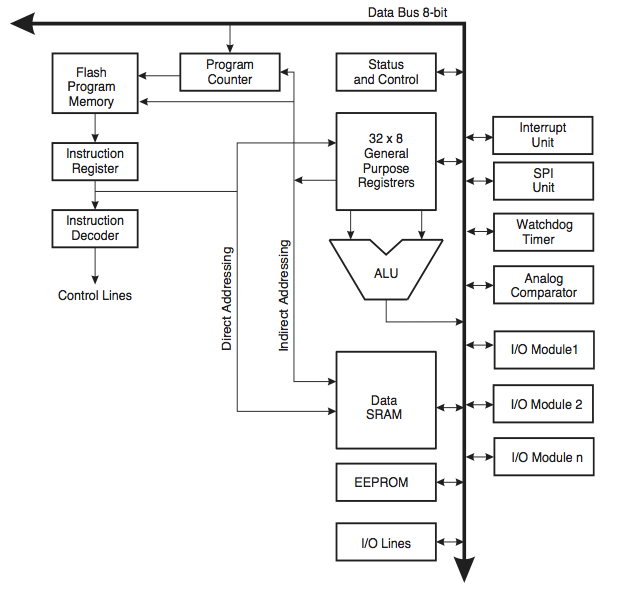
\includegraphics[width=400px,height=385px]{pictures/avr.png}
		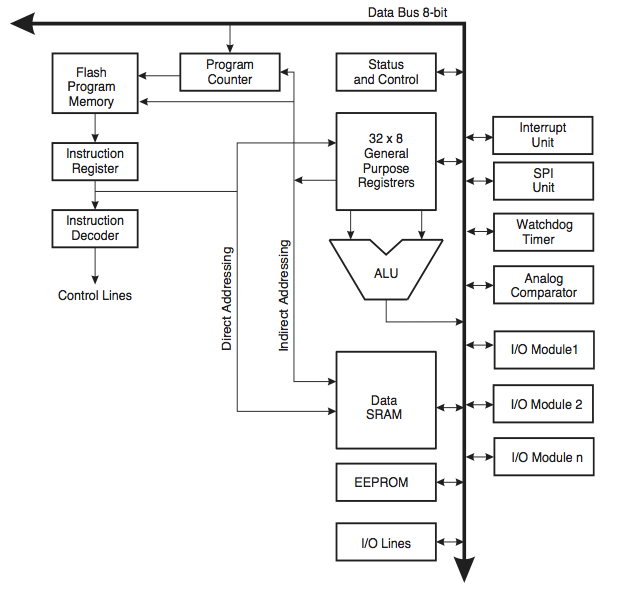
\includegraphics[width=360px,height=355px]{pictures/avr.png}
	}
	\caption[AVR-Architektur]{AVR-Architektur \cite{Atmel:ATMega16}}\label{fig:avr}
\end{figure}

%%%%%%%%%%%%%%%%%%%%%%%%%%%%%%%%%%%%%%%%%%%%%%%%%%%%%%%%%%%%%%%%%%%%%%%%%%%%%%%
\subsection{Timer-Einheit}

Der Timer ist eine Einheit im Mikrocontroller, die einen Zähler enthält und diesen Zähler periodisch inkrementiert und/oder dekrementiert. Unmittelbar nach dem Auftreten eines Ereignisses wird das Hauptprogramm unterbrochen, wobei diese Unterbrechung meist mit dem englischen Begriff \textit{Interrupt} bezeichnet wird. Eine spezielle Art des Interrupts ist das Timer-Interrupt, weil speziell eingestellt werden kann, wann der Interrupt ausgelöst werden soll. Genau genommen ist ein Timer-Interrupt auch ein Zustand\footnote{Wenn der Interrupt auslöst, wird diese Stelle markiert, wobei diese Markierung als \textit{Zeitstempel} in Echtzeit bezeichnet wird.} des Zählers. Grundsätzlich wird der Timer-Interrupt genau dann ausgelöst, wenn der Wert des Zählers einen vordefinierten Wert erreicht oder ein externes Ereignis an einem Pin des Mikrocontrollers auftritt. Der ATMega16-Mikrocontroller hat drei verschiedene unabhängige Timer-Einheiten, wobei zwei mit 8-Bit und ein mit 16-Bit-Auflösung. 

%%%%%%%%%%%%%%%%%%%%%%%%%%%%%%%%%%%%%%%%%%%%%%%%%%%%%%%%%%%%%%%%%%%%%%%%%%%%%%%
\subsubsection{CTC-Modus}

In dieser Arbeit wurde der 16-Bit Timer/Counter1 ausgewählt und dieser wurde im CTC-Modus konfiguriert. In diesem Modus wird der Timer-Interrupt nur dann ausgelöst, wenn der Zähler (\textit{TCNT1}\footnote{Der Timer/Counter\textbf{1}-Zähler ist ein 16-Bit Register und enthält untereinander geschachtelte \textbf{LOW} (\textit{TCNT1L}) und \textbf{HIGH} (\textit{TCNT1H}) Bytes.}) den maximalen Wert (\textit{TOP}) erreicht. Anschließend fängt er wieder bei dem Wert (\textit{BOTTOM}) an (siehe \autoref{fig:timer}). \smallskip \smallskip

\begin{figure}[htbp]
	\centering
	\fbox{
		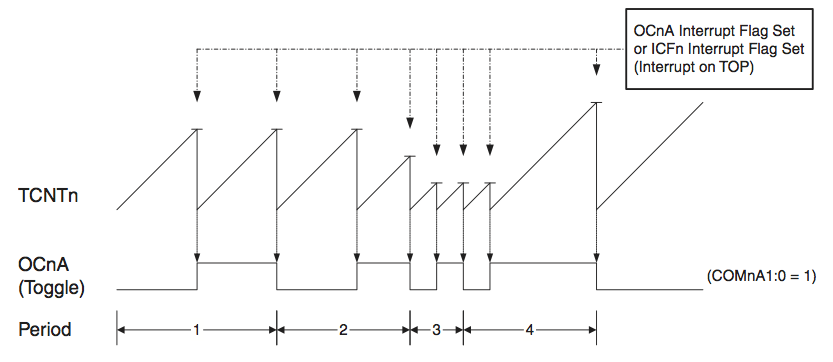
\includegraphics[width=450px,height=195px]{pictures/timer.png}
	}
	\caption[Timer-Diagramm für CTC-Mode]{Timer-Diagramm für CTC-Mode \cite{Atmel:ATMega16}}\label{fig:timer}
\end{figure}
\smallskip \smallskip

%\newpage
Zum Konfigurieren des Timer/Counter1 gibt es zwei Steuerregister, wie in \autoref{tab:tccr1a} und \autoref{tab:tccr1b} beschrieben wird. \smallskip \smallskip

\begin{table}[htbp]
	\centering
	\begin{tabular}{ |c|c|c|c|c|c|c|c|} \hline
		COM1A1 & COM1A0 & COM1B1 & COM1B0 & FOC1A & FOC1B & WGM11 & WGM10 \\ \hline
	\end{tabular}
	\caption{Timer/Counter1 Controler Register A (TCCR1A)}\label{tab:tccr1a}
\end{table}

\begin{table}[htbp]
	\centering
	\begin{tabular}{ |c|c|c|c|c|c|c|c|} \hline
		ICNC1 & ICES1 & (reserviert) & WGM13 & WGM12 & CS12 & CS11 & CS10 \\ \hline
	\end{tabular}
	\caption{Timer/Counter1 Controler Register B (TCCR1B)}\label{tab:tccr1b}
\end{table}

Jedes Bit an den Steuerregistern hat eine spezifische Aufgabe. Änderungen an diesen Bits rufen verschiedene Timer-Modi auf. Bei einem Timer sind verschiedenste Kombinationen möglich, welche im Datenblatt vom ATMega16 zu entnehmen ist. \smallskip \smallskip

Die zwei Byte Steuerregister des Timer/Counter1 sind wie folgt konfiguriert:

\begin{itemize}
	\item CTC-Modus
	\item Der Zähler wurde periodisch in 1 $HZ$ beschränkt.
	\item Input-Capture Noise Canceler
	\item Der Vorteiler wurde mit \textit{256}\footnote{Dies bedeutet, dass der Systemtakt um den Faktor $256$ geteilt wird.} gewählt.
\end{itemize}

%%%%%%%%%%%%%%%%%%%%%%%%%%%%%%%%%%%%%%%%%%%%%%%%%%%%%%%%%%%%%%%%%%%%%%%%%%%%%%%
\subsubsection{Input Capture}

Input Capture ist ein Hardwareteil, der zur genaueren Zeitmessung dient. Das Eingangssignal muss an den ICP angeschlossen werden, um eine Messung durchzuführen. Angewendet wird der Input Capture zwischen zwei aufeinanderfolgende Flanken, wobei die Erkennung entweder auf steigende oder fallende Flanken basiert. \smallskip \smallskip

Der Zähler läuft genau wie im CTC-Modus vom BOTTOM- zum TOP-Wert. Wenn eine eingestellte Zustandsänderung (fallende oder steigende Flanken) am ICP auftritt, wird der aktuelle Zählerwert auf eine Variable übergeben. Bei der nächsten Zustandsänderung wird die Differenz zwischen dem aktuellen Zählerwert und dem zuvor kopierten Zählerwert ermittelt. Diese Differenz ist die Messung zwischen zwei aufeinanderfolgenden Zustandsänderungen. Dieses Szenario findet bei jeder positiven bzw. negativen Flanke fortlaufend statt. 

%%%%%%%%%%%%%%%%%%%%%%%%%%%%%%%%%%%%%%%%%%%%%%%%%%%%%%%%%%%%%%%%%%%%%%%%%%%%%%%
\subsection{SPI-Schnittstelle}
% http://www.uni-koblenz.de/~physik/informatik/MCU/SPI.pdf
% http://www.weigu.lu/a/pdf/MICEL_C4_SPI.pdf
% http://www.netzmafia.de/skripten/hardware/Control/schnittstellen.pdf
% http://wiki.attraktor.org/images/d/d4/Arduino_stammtisch-serielle_kommunikation_spi.pdf
% http://gedankenlyrik.bplaced.net/www/studium/seminararbeit_2008.pdf
% http://avrbeginners.net/architecture/spi/spi.html

Die SPI-Schnittstelle ist ein Bus-System, welches synchron serielle Daten überträgt und von der Firma Motorola entwickelt wurde. Die Funktionsweise basiert auf dem Master-Slave-Prinzip. Die SPI-Schnittstelle unterstützt den richtungsunabhängigen (Full Duplex\footnote{Daten können in beide Richtungen gleichzeitig übertragen werden.}) Nachrichtenaustausch. Die einfache Master-Slave-Verbindung kann wie in der \autoref{fig:spi} hergestellt werden. \smallskip \smallskip

Das Master-Slave-Prinzip ist eine Zugriffsform, bei welcher die höchste Priorität am Bus zu schreiben beim Master liegt. Außerdem entscheidet der Master über den gemeinsam genutzten Übertragungskanal, bei welcher ein oder mehrere Slaves auch angeschlossen sind. Dies führt dazu, dass wenn der Slave den Bus verwenden möchte, muss er warten, dass der Master ihn auffordert, Daten zu senden bzw. zu empfangen. Dieses Prinzip wird sehr oft auch \textit{zentrales Polling}\footnote{Der Master fragt ununterbrochen die Slaves an, ob sie den Bus benötigen.} genannt. \smallskip \smallskip

\begin{figure}[htbp]
	\centering
	\fbox{
		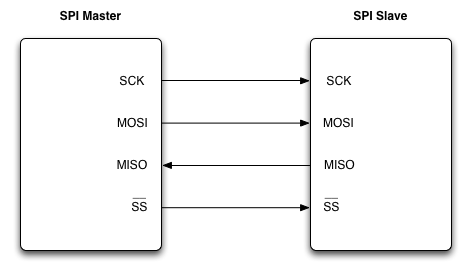
\includegraphics[width=345px,height=200px]{pictures/spi.png}
	}
	\caption{SPI-Verbindung zwichen einem Master und einem Slave}\label{fig:spi}
\end{figure}

Der Übertragungstakt wird vom Master erzeugt und über die Ausgangsleitung (\textit{SCK}-Pin) an alle Slaves geleitet. Im Master-Betrieb muss der SCK-Pin (\textit{PB7}) des ATMega16-Mikrocontrollers als Ausgang eingestellt werden. Im Gegensatz muss der SCK-Pin im Slave-Betrieb als Eingang konfiguriert werden. Dabei wird der $\overline{SS}$-Pin \textbf{LOW} gesetzt, damit der Slave zum Empfangen bereit gestellt wird. Die wichtigste Pins und deren Initialisierungen im Master- und Slave-Betrib werden in der folgenden \autoref{spi:pins} beschrieben: \smallskip \smallskip

\begin{table}[htbp]
	\centering
	\begin{tabular}{ |c|c|c| } \hline
		Pin & Master-Betrieb & Slave-Betrieb \\ \hline \hline
		MOSI & als Ausgang zu initialisieren & automatisch Eingang \\ \hline
		MISO & automatisch Eingang & als Ausgang zu initialisieren \\ \hline
		SCK & als Ausgang zu initialisieren & automatisch Eingang \\ \hline
		$\overline{SS}$ & als Ausgang zu initialisieren & automatisch Eingang \\ \hline
	\end{tabular}
	\caption{Initialisierung von SPI-Pins}\label{spi:pins}
\end{table}

%%%%%%%%%%%%%%%%%%%%%%%%%%%%%%%%%%%%%%%%%%%%%%%%%%%%%%%%%%%%%%%%%%%%%%%%%%%%%%%
\subsection{Debugging}

Bei der Programmierung ist es sehr wichtig zu wissen, in welchem Zustand das Programm sich gerade befindet. Dies erleichtert das Debugging erheblich, da bei jeder Programmabzweigung beispielsweise eine Led eingeschaltet werden kann. Durch das gezielte Ein- bzw. Ausschalten der Leds wird genau erkannt, welchen Pfad das Programm durchläuft. In dieser Arbeit wurde PORTA zum Debugging ausgewählt, an den die Leds verbunden sind. Es können nur so viele Leds als Ausgang dienen, so viele auch als Ausgänge definiert werden. Beispielsweise ist es sehr hilfreich, wenn eine Led für ein bestimmtes Ereignis (z.B. Timer-Interrupt) abwechselnd ein- bzw. ausgeschaltet wird (\textit{toggle}). 

%%%%%%%%%%%%%%%%%%%%%%%%%%%%%%%%%%%%%%%%%%%%%%%%%%%%%%%%%%%%%%%%%%%%%%%%%%%%%%%
\section{Netzwerk-Modul}\label{sec:network}

Damit zwei oder mehrere Geräte miteinander verbunden werden können, um gegenseitig Daten auszutauschen, wird eine Kommunikationsschnittstelle benötigt. Die Kommunikationsschnittstelle baut ein Übertragungskanal zwischen den kommunizierenden Geräten auf. Heutzutage gibt es viele Kommunikationsprotokolle mit verschiedenen Austauschstrategien auf unterschiedlichen Kommunikationsebene. Die Praxis zeigt, dass zwischen den Computern sehr oft das Ethernet-Kanal in Verwendung kommt. Die Vernetzung, welche auf Ethernet-Kanal basiert, wird als LAN bezeichnet. Dieses wird verwendet, um in einem lokalen Netz höhere Datenraten zu erzielen. \smallskip \smallskip

Im nächsten Kapitel werden mehrere Kommunikationsprotokolle näher beschrieben. Dabei wird sowohl der Aufbau als auch die Funktionsweise der einzelnen Schichten der Kommunikationsprotokolle aufgezählt. Auch die hardwarenahe Realisierung des Aufbaus und die Anordnung des Speichermoduls finden in diesem Unterkapitel Platz. 

%%%%%%%%%%%%%%%%%%%%%%%%%%%%%%%%%%%%%%%%%%%%%%%%%%%%%%%%%%%%%%%%%%%%%%%%%%%%%%%
\subsection{Aufbau}
% http://www.rn-wissen.de/index.php/ENC28J60
Der Hersteller \textit{Mikrochip Technology Inc} \cite{Microchip} produziert sehr effiziente Mikrochips für Ethernets. Auch in dieser Arbeit wurde ein Mikrochip dieses Herstellers verwendet, und zwar das Modell \textbf{ENC28J60} \cite{Microchip:ENC28J60}. Dieser Mikrochip ist ein \textit{IEEE 802.3} \cite{IEEE:802.3} kompatibler Ethernet-Controller. \smallskip \smallskip

\begin{figure}[htbp]
	\centering
	\fbox{
		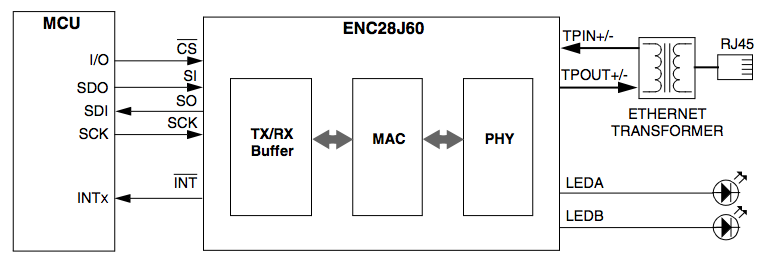
\includegraphics[width=450px,height=155px]{pictures/enc28j60.png}
	}
	\caption[Basisverbindungen zwischen dem ENC28J60 und einem Mikrocontroller]{Basisverbindungen zwischen dem ENC28J60 und einem Mikrocontroller \cite{Microchip:ENC28J60:Datasheet}}\label{fig:enc28j60}
\end{figure}

Der ENC28J60-Mikrochip ist im Gegensatz zu anderen Ethernet-Controllern ein kleiner Chip mit 28-Pins und besitzt einen kleinen Speicher. Es wurde gezielt dieser Mikrochip verwendet, da die Einfachheit und Übersichtlichkeit bei der Laboranwendungen nicht verloren geht. \smallskip \smallskip %Als Nachteil gilt der relativ hohe Stromverbrauch, welche jedoch keine große Relevanz für diese Arbeit hat. \\

Verglichen mit anderen Netzwerk-Mikrochips ist der ENC28J60 klein und dementsprechend auch sehr einfach, ihn in Schaltungen einzubauen. Er enthält eine SPI-Schnittstelle und kann über sie von einem Mikrocontroller leicht angesteuert werden. Die Programmierung der SPI-Schnittstelle ist sowohl im Vollduplex- als auch im Halbduplex-Modus möglich. Allein durch Basisverbindungen des Moduls ist die Funktion gegeben. Wie in der \autoref{fig:enc28j60} zu erkennen ist, handelt sich bei den Basisverbindungen um einige wenige Pins. \smallskip \smallskip

Weiters bietet der ENC28J60 folgende charakteristische Eigenschaften:

\begin{itemize}
	\item integrierten MAC
	\item 10 $MBit/s$ Ethernet-Schnittstelle (10BASE-T Physical Layer)
	\item Voll-/Halb-Dublex Datenverkehr
	\item 8 Kilobytes internen Puffer
	\item SPI-Takt bis zu 25 MHz
\end{itemize}

Um mit einem Rechner im LAN zu kommunizieren, muss der ENC28J60-Mikrochip an eine Ethernet-Buchse angeschlossen werden, wie in der \autoref{fig:enc28j60} dargestellt wurde. Es wird ein festes Kommunikationskabel zwischen dem ENC28J60-Mikrochip und einem Server verlegt. Um das Ethernetkabel an die Buchse anzustecken, wird eine RJ45-Netzwerkstecker benötigt, welcher ein standardisierter Modularstecker ist. Für die \textbf{10BASE-T}-Kommunikation werden nicht alle Adernpaare benötigt. Belegt sind nur zwei Adernpaare, wobei das erste Adernpaar für den Datenausgang und das zweite für den Dateneingang verwendet werden. Diese Adernpaare besitzen je zwei Pins, wobei immer je ein positives und ein negatives Pin für das Eingangs- bzw. Ausgangssignal benötigt werden (siehe \autoref{tab:rj45}). Die Verdrahtung zwischen der RJ45-Buchse und dem ENC28J60-Mikrochip wurde in der \autoref{fig:ethernet} dargestellt. \smallskip \smallskip

\begin{table}[htbp]
	\centering
	\begin{tabular}{ |c|c|c|c| } 
	\hline
		PIN & Signal & Beschreibung & Farbe \\ \hline
		1 & TX+ & positive Sendedaten & weiß/grün \\ \hline
		2 & TX- & negative Sendedaten & grün \\ \hline
		3 & RX+ & positive Empfangsdaten & weiß/orange \\ \hline
		4 & nicht belegt &  & blau \\ \hline
		5 & nicht belegt &  & weiß/blau\\ \hline
		6 & RX- & negative Empfangsdaten & orange \\ \hline
		7 & nicht belegt &  & weiß/orange \\ \hline
		8 & nicht belegt &  & braun \\ \hline
	\end{tabular}
	\caption{Pinbelegung von RJ45-Modularbuchse bzw. -stecker \cite{RJ45:Pins}}\label{tab:rj45}
\end{table}

\begin{table}[htbp]
\centering
\begin{tabular}{ |c|c|c|c| }
  \hline
  \multicolumn{2}{|c|}{\textbf{ENC28J60}} & \multicolumn{2}{|c|}{\textbf{RJ45-Buchse}}\\ 
  \hline
  PIN17 & TPOUT+ & TX+ & 1 \\
  PIN16 & TPOUT- & TX- & 2 \\
  PIN13 & TPIN+ & RX+ & 3 \\
  PIN12 & TPIN- & RX- & 6 \\
  \hline
\end{tabular}
\caption{Verdrahtung zwischen dem RJ45-Buchse und dem ENC28J60-Mikrochip}\label{fig:ethernet}
\end{table}

Wie in der \autoref{fig:enc28j60} zu sehen ist, wird der ENC28J60-Mikrochip nach der Verdrachtung mit dem ATMega16-Mikrocontroller über $\overline{\textbf{CS}}$ ausgewählt werden kann. Die Daten werden über den \textbf{SI}-Pin und über den \textbf{SO}-Pin ein- bzw. ausgelesen, welche mit dem \textbf{SCK} (Takt) von dem Mikrocontroller über die Synchron-Serielle Schnittstelle gesteuert werden können. Mit dem $\overline{\textbf{INT}}$-Pin gibt es eine Möglichkeit zu merken, ob ein passendes Ethernetpaket eingetroffen ist. \smallskip \smallskip

Außerdem besitzt der ENC28J60-Mikrochip zwei Pins (\textit{PIN26} und \textit{PIN27}) für die Leds. Während dem Datenempfang blinkt die \textit{LEDB} und die \textit{LEDA} während der Datensendung. Diese Funktion ist gegeben, wenn die Buchse sie unterstützt. Ansonsten können diese zwei Leds seperat verdrahtet werden, damit das Debugging beim Datenaustausch erleichtert wird. 

%%%%%%%%%%%%%%%%%%%%%%%%%%%%%%%%%%%%%%%%%%%%%%%%%%%%%%%%%%%%%%%%%%%%%%%%%%%%%%%
\subsection{Speicheranordnung}
Der Gesamtspeicher des ENC28J60-Mikrochips wird als statisches RAM implementiert. Der Speicher wurde in drei Teile unterteilt, welche \textbf{Steuerregister}, \textbf{Ethernet-Puffer} und \textbf{PHY-Register} genannt werden, wie in der \autoref{fig:enc28j60_memory} zu sehen ist.  \smallskip \smallskip

\begin{figure}[htbp]
	\centering
	\fbox{
		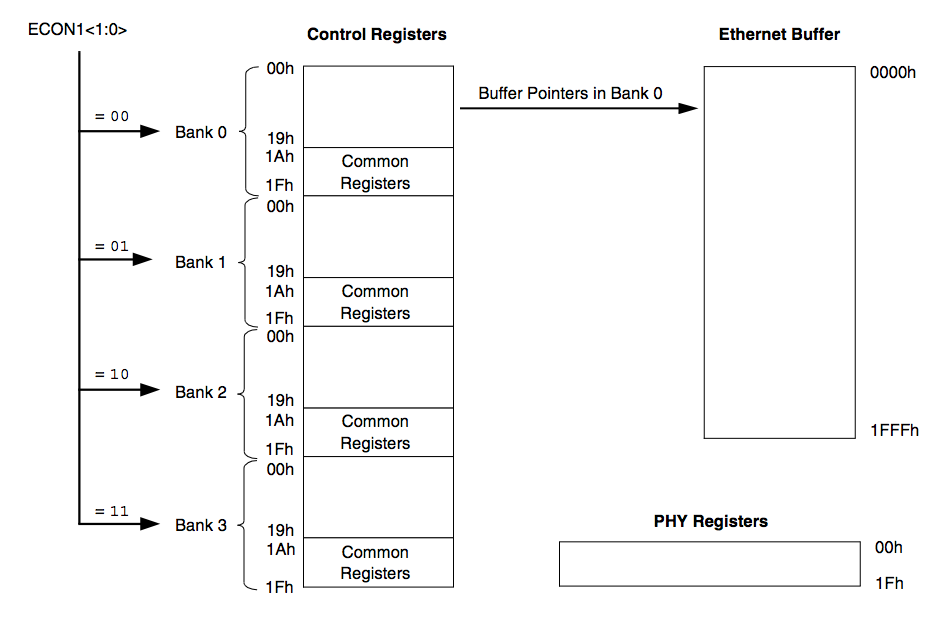
\includegraphics[width=425px,height=280px]{pictures/enc28j60_memory.png}
	}
	\caption[Speicheranordnung des ENC28J60-Mikrochips]{Speicheranordnung des ENC28J60-Mikrochips \cite{Microchip:ENC28J60:Datasheet}}\label{fig:enc28j60_memory}
\end{figure}

Das Steuerungsregister (Control Register) bildet die wichtigste Schnittstelle zwischen dem Mikrocontroller und ENC28J60-Mikrochip. Die Aufgaben des Steuerregisters sind die Konfiguration, die Steuerung und die Überwachung des Mikrochips. Das Steuerregister enthält vier Bänke untereinander. Jede Bank hat eine Größe von 32-Bit. Die letzten fünf Register (von $1B$ bis $1F$) jeder Bank weisen auf die gleichen Registernamen. Sie sind Schlüsselregister, welche als Steuerung bzw. Überwachung des Mikrochips verwendet werden. Um die aktive Bank auszuwählen, wird der \textbf{ECON1<1:0>} (sog. Common Register) eine von vier Kombinationen ($00$, $01$, $10$ oder $11$) für die Bänke gesetzt. \smallskip \smallskip

\begin{figure}[htbp]
	\centering
	\fbox{
		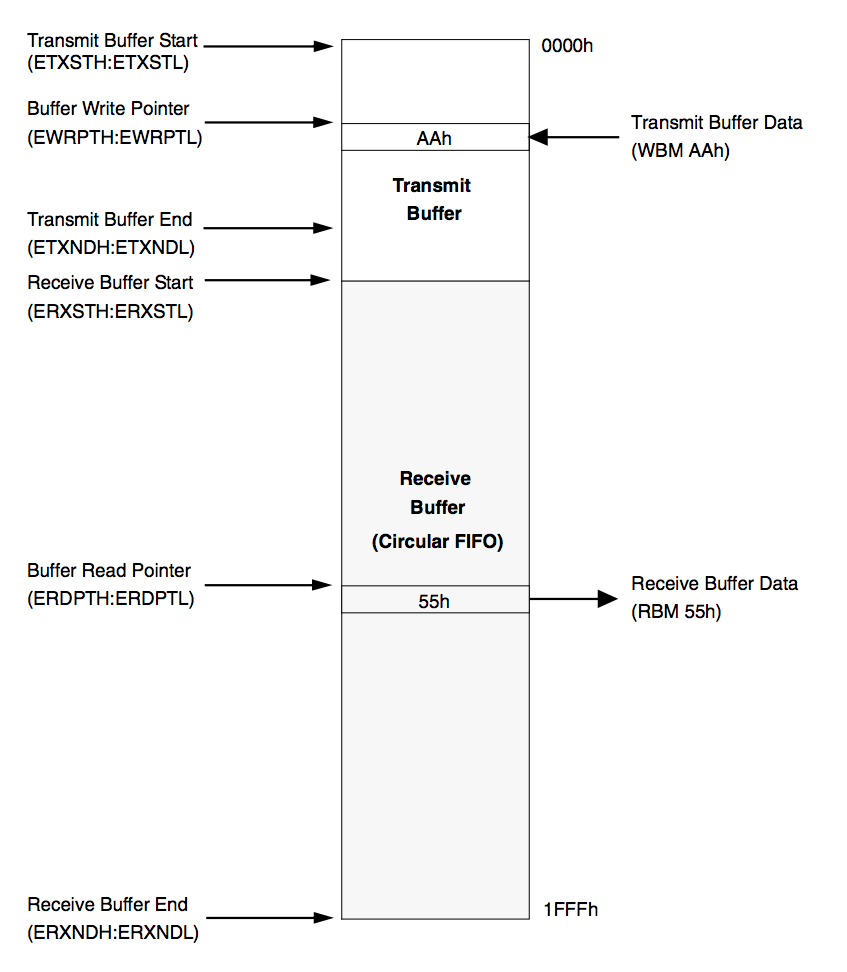
\includegraphics[width=330px,height=380px]{pictures/enc28j60_puffer.png}
	}
	\caption[Pufferanordnung des ENC28J60-Mikrochips]{Pufferanordnung des ENC28J60-Mikrochips \cite{Microchip:ENC28J60:Datasheet}}\label{fig:enc28j60_puffer}
\end{figure}

ENC28J60-Mikrochip hat 8 KB Pufferspeicher. Die erste vier Register der Bank-0 sind Zeiger auf die Adresse des Pufferspeichers, welche zum Lesen und Schreiben gedacht sind. Der Puffer ist unterteilt in zwei, nämlich in Empfangspuffer und Sendepuffer. Die Größe des Sendepuffers ist abhängig von der Größe des Empfangspuffers. Umso größer der Empfangspuffer ist, desto kleiner ist der Sendepuffer. Als Sendepuffer wird dieser Bereich im Speicher bezeichnet, welcher nicht für den Empfang benötigt wird. Die empfangene Daten werden im Empfangspuffer nach dem FIFO-Prinzip (Ringwarteschleife) abarbeitet. Die gesamte Pufferandordung wurde in der \autoref{fig:enc28j60_puffer} dargestellt. \smallskip \smallskip

Um das PHY-Modul zu konfigurieren, wird das \textbf{PHY-Register} verwendet, welches verfügbare 16-Bit beinhaltet. Wegen den Sicherheitsgründen gibt es keinen direkten Zugang über die SPI-Schnittstelle zu diesem Register. Stattdessen wird der Zugang durch einen speziellen Satz von MAC-Steuerregister erzielt.

% http://ww1.microchip.com/downloads/en/AppNotes/00833c.pdf
% http://michaelmoetz.mi.funpic.de/da/datenblaetter/Ethernet_Theory_of_Operation_(Microchip_AN1120)(2008).pdf



